%%%%%%%%%%%%%%%%%%%%%%%%%%%%%%%%%%%%%%%%%
% University Assignment Title Page 
% LaTeX Template
% Version 1.0 (27/12/12)
%
% This template has been downloaded from:
% http://www.LaTeXTemplates.com
%
% Original author:
% WikiBooks (http://en.wikibooks.org/wiki/LaTeX/Title_Creation)
%
% License:
% CC BY-NC-SA 3.0 (http://creativecommons.org/licenses/by-nc-sa/3.0/)
% 
% Instructions for using this template:
% This title page is capable of being compiled as is. This is not useful for 
% including it in another document. To do this, you have two options: 
%
% 1) Copy/paste everything between \begin{document} and \end{document} 
% starting at \begin{titlepage} and paste this into another LaTeX file where you 
% want your title page.
% OR
% 2) Remove everything outside the \begin{titlepage} and \end{titlepage} and 
% move this file to the same directory as the LaTeX file you wish to add it to. 
% Then add \input{./title_page_1.tex} to your LaTeX file where you want your
% title page.
%
%%%%%%%%%%%%%%%%%%%%%%%%%%%%%%%%%%%%%%%%%
%\title{Title page with logo}
%----------------------------------------------------------------------------------------
%	PACKAGES AND OTHER DOCUMENT CONFIGURATIONS
%----------------------------------------------------------------------------------------

\documentclass[12pt]{article}
\usepackage[italian]{babel}
\usepackage[utf8x]{inputenc}
\usepackage{amsmath}
\usepackage{graphicx}
\usepackage[colorinlistoftodos]{todonotes}
\usepackage{float}

\begin{document}

\begin{titlepage}

\newcommand{\HRule}{\rule{\linewidth}{0.5mm}} % Defines a new command for the horizontal lines, change thickness here

\center % Center everything on the page
 
%----------------------------------------------------------------------------------------
%	HEADING SECTIONS
%----------------------------------------------------------------------------------------

\textsc{\LARGE Università degli studi di Milano-Bicocca}\\[1cm] % Name of your university/college
\textsc{\Large Advanced Machine Learning }\\[0.3cm] % Major heading such as course name
\textsc{\large Progetto Finale}\\[0.1cm] % Minor heading such as course title

%----------------------------------------------------------------------------------------
%	TITLE SECTION
%----------------------------------------------------------------------------------------

\HRule \\[0.4cm]
{ \huge \bfseries PetFinder.my - Un Approccio Ibrido}\\[0.4cm] % Title of your document
{ \large \textbf{Predizione Della Popolarità Di Foto Di Animali}}
\HRule \\[1.5cm]
 
%----------------------------------------------------------------------------------------
%	AUTHOR SECTION
%----------------------------------------------------------------------------------------

\large
\emph{Autori:}\\
Francesco Lenti - 865274 - f.lenti3@campus.unimib.it \\   % Your name
Mattia Boller - 873358 - m.boller@campus.unimib.it   \\
Mattia Marchi - 817587 - m.marchi@campus.unimib.it   \\[1cm] % Your name

% If you don't want a supervisor, uncomment the two lines below and remove the section above
%\Large \emph{Author:}\\
%John \textsc{Smith}\\[3cm] % Your name

%----------------------------------------------------------------------------------------
%	DATE SECTION
%----------------------------------------------------------------------------------------

{\large \today}\\[1cm] % Date, change the \today to a set date if you want to be precise

%----------------------------------------------------------------------------------------
%	LOGO SECTION
%----------------------------------------------------------------------------------------


\includegraphics[scale=0.85]{logo.png}\\ % Include a department/university logo - this will require the graphicx package
 
%----------------------------------------------------------------------------------------

\vfill % Fill the rest of the page with whitespace

\end{titlepage}


\begin{abstract}
    Una immagine vale più di mille parole. Sapevi che un' immagine può salvare più di mille vite? Milioni di animali randagi soffrono per le strade o vengono soppressi nei rifugi ogni giorno in tutto il mondo. È chiaro aspettarsi che gli animali con foto più "attraenti" generino più interesse e vengano adottati più velocemente. Ma cosa rende "attraente" una immagine? Con l'aiuto del Deep Learning si è cercato di determinare l'attrattiva di una foto di un animale al fine di dargli una maggiore possibilità di adozione. In questo documento sono illustrate le tecniche e le soluzioni adottate, tramite l'unione di diversi modelli di deep neural network, per ottenere tale score di popolarità. 
\end{abstract}

\section{Introduzione}
    Il task fa riferimento ad una competizione aperta su Kaggle \footnote{https://www.kaggle.com/c/petfinder-pawpularity-score}.
    La competizione è finanziata da PetFinder.my, principale piattaforma per il benessere degli animali della Malesia. Attualmente, PetFinder.my utilizza un misuratore per stimare la popolarità delle foto di animali randagi ospitati all'interno di rifugi. Questo misuratore analizza le statistiche riguardanti il traffico generato dalle foto degli animali, presenti su diversi portali, e ne stima la popolarità. Sebbene questo strumento sia utile, potrebbe essere ancora migliorato. L'obiettivo finale è quello di stimare a priori la "Pawpularity" (termine coniato dalla piattaforma per indicare la popolarità di una foto) di un animale in base alla foto del suo profilo, in modo di scegliere quelle che ne faciliterebbero l'adozione. Insieme alle foto di migliaia di animali vengono anche forniti dei metadati, etichettati a mano, per ogni foto. Vengono forniti quindi due dataset, uno con le foto degli animali e l'altro con i corrispettivi metadati.
    La soluzione proposta utilizza un modello multi-input, per utilizzare tutte le informazioni a disposizione. Da un lato una rete convoluzionale che sfrutta un approccio di fine-tuning basato su transfer learning, dall'altro una semplice rete neurale fully-connected. Gli output delle due reti vengono concatenati e processati da un ulteriore layer fully-connected finale per ottenere l'output, ovvero il Pawpularity score.


\section{Dataset}
    Vengono forniti un dataset di immagini e un dataset tabulare contenente i metadati delle immagini.\\ In particolare, i dati di training comprendono:
    \begin{itemize}
        \item Una cartella \textbf{train} contenente 9912 immagini di training nella forma \textit{\{id\}.jpg}, dove id è un identificativo univoco del profilo dell'animale;
        \item Un file \textbf{\textit{train.csv}} contenente i metadati e il Pawpularity score per ogni immagine.
    \end{itemize}

    I dati di testing non sono disponibili, dato che si tratta di una competizione Kaggle ancora aperta al momento della stesura di questo report. Tuttavia, vengono fornite la cartella \textbf{test} e il file \textbf{\textit{test.csv}} di 8 immagini al fine di testare la submission dell'algoritmo.
    Inoltre è presente anche un file \textbf{\textit{sample\_submission.csv}} con un esempio di submission. Dopo aver inviato la submission, il modello verrà testato su un subset pari al 25\% del dataset originale di test, contenete circa 6800 immagini, il quale verrà utilizzato solo al termine della competizione per stilare la classifica finale.

    
    \subsection{Esplorazione Dataset}
    Processo per investigare quelle che sono le caratteristiche chiave dei dataset. Prima di costruire un modello di machine learning è necessario capire il dataset con cui si sta lavorando e il problema che si sta cercando di risolvere.

    \subsubsection{Immagini}
    Per quanto riguarda il dataset delle immagini si andrà a mostrare alcune foto in base al pawpularity score assegnato.
    Si analizzano quindi le immagini, partendo dai voti più bassi andando verso quelli più alti. Per non rendere il report troppo prolisso, sono stati inseriti solo 3 gradi di pawpularity: 1, 50 e 100, il resto dell'analisi è disponibile nel notebook.
    
    \begin{figure}[H]
        \centering
        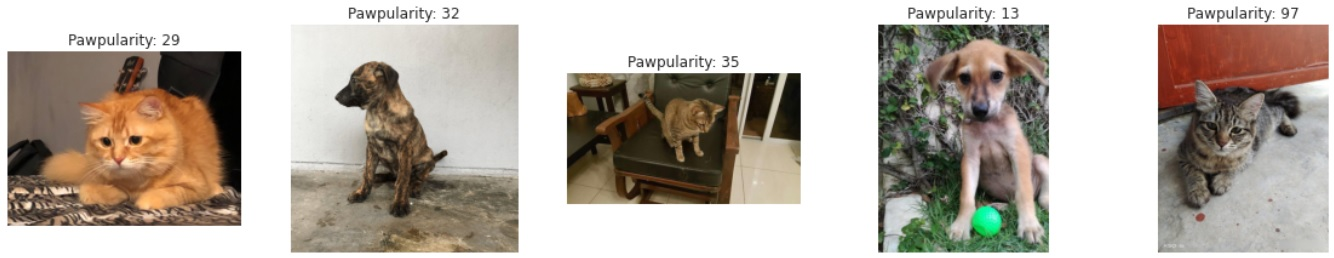
\includegraphics[scale=0.7]{Plot/pawpularity_preview.jpg}
        \caption{Confronto animali con diversa pawpularity}
        \label{fig:paw_10}
    \end{figure}

    Dall'analisi visiva effettuata non si evincono particolari dettagli su cosa possa rendere una foto più "popolare" rispetto ad un'altra, è facile, infatti, trovare delle belle foto di animali con score di pawpularity sotto il 10.

    \subsubsection{Metadati}
    Come descritto in precedenza il file \textit{train.csv} contiene i metadati per ogni immagine. In figura \ref{fig:target} viene visualizzata la distribuzione del target, ovvero il Pawpularity score.
    \begin{figure}[H]
        \centering
        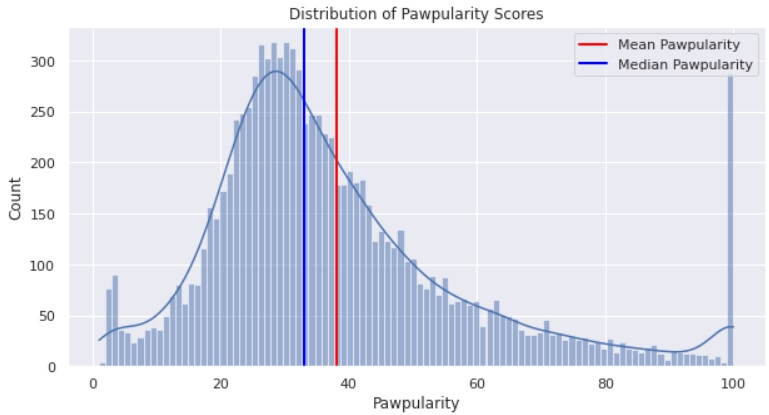
\includegraphics[scale=0.6]{Plot/distribution_target.jpg}
        \caption{Distribuzione dello score di Pawpularity}
        \label{fig:target}
    \end{figure}

    Si può osservare come la distribuzione dello score sia concentrata principalmente tra i valori 20 e 50 con una forte presenza di immagini con score uguale a 100.
    Successivamente è stata analizzata la distribuzione del target per ogni singola feature del dataset.
    Per fare ciò si utilizzano degli istogrammi, mostrando il Pawpularity score sull'asse x e la somma dei valori di ogni feature sull'asse y. Questo può aiutare a comprendere se alcune feature impattano più di altre nel calcolo del Pawpularity score.

    \begin{itemize}
        \item \textbf{Occlusion} - Oggetti indesiderati che bloccano una parte dell'animale. Nota: Non tutti gli oggetti bloccanti sono considerati occlusione;
        \begin{figure}[H]
            \centering
            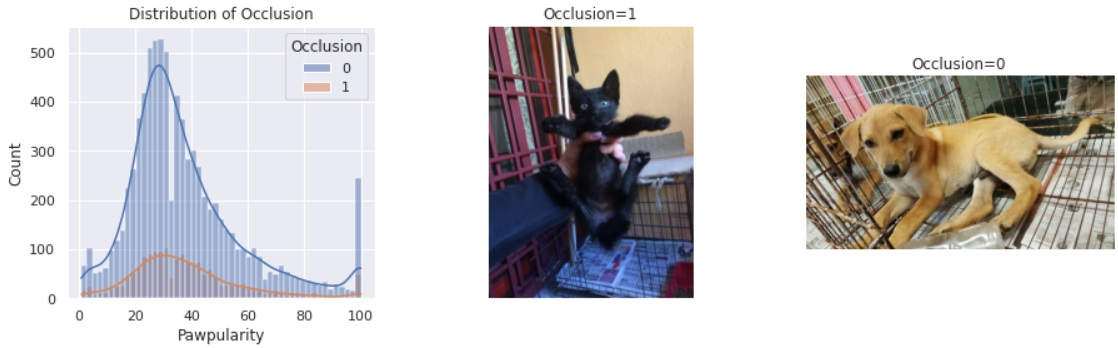
\includegraphics[scale=0.5]{Plot/distribution_occlusion.jpg}
            \caption{Distribuzione ed esempio della feature Occlusion}
            \label{fig:occlusion}
        \end{figure}
        \item \textbf{Action} - Animale nel mentre di un'azione (ad es. saltare);
        \begin{figure}[H]
            \centering
            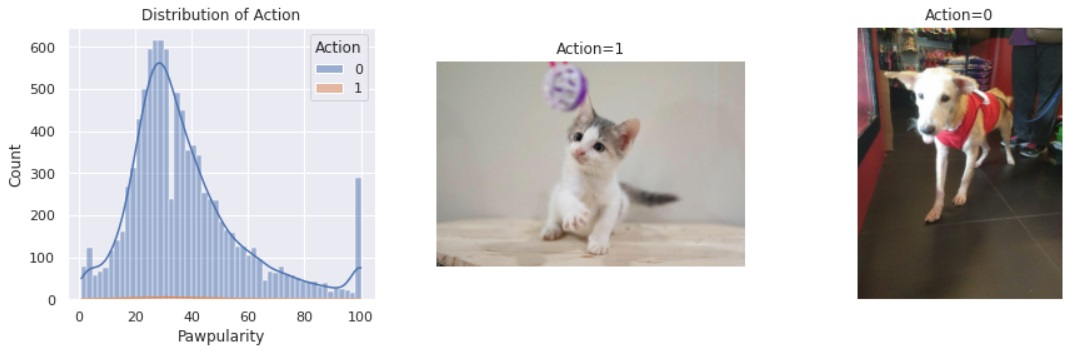
\includegraphics[scale=0.5]{Plot/distribution_action.jpg}
            \caption{Distribuzione ed esempio della feature Action}
            \label{fig:action}
        \end{figure}
        \item \textbf{Near} - Singolo animale che occupa una porzione significativa della foto (circa oltre il 50\% della larghezza o dell'altezza della foto);
        \item \textbf{Focus} - L'animale è posizionato su uno sfondo ordinato, non troppo vicino/lontano;
        \item \textbf{Eyes} - Entrambi gli occhi sono rivolti verso l'obiettivo, con almeno un occhio/pupilla decentemente chiaro;
        \item \textbf{Face} - Viso discretamente chiaro e rivolto in avanti;
        \item \textbf{Accessory} - Accessorio/oggetto di accompagnamento fisico o digitale, come un giocattolo o un adesivo digitale, esclusi collare e guinzaglio;
        \item \textbf{Group} - Più di 1 animale nella foto;
        \item \textbf{Collage} - Foto ritoccata digitalmente;
        \item \textbf{Human} - Umano nella foto;
        \item \textbf{Info} - Mesto o etichette personalizzati (ad es. nome dell'animale, descrizione);
        \item \textbf{Blur} - Notevolmente sfocato o rumoroso, soprattutto per gli occhi e il viso dell'animale. Per le voci Sfocatura, la colonna "Occhi" è sempre impostata su 0.
    \end{itemize}
    

\section{Approccio metodologico}

    La competizione proposta da PetFinder.my si presenta come un problema di regressione, con l'obiettivo di creare un modello capace di assegnare un punteggio di attrattività, 
    compreso tra 0 e 100, ad una determinata foto di un animale.
    Nei seguenti paragrafi verrano presentati i vari step che hanno portato alla definizione del modello finale utilizzato per il task sopra descritto.
    Si è partiti da alcuni modelli di deep learning più tradizionali, quali fully-connected neural networks e convolutional neural networks, per poi cercare di combinare le informazioni
    contenute nelle immagini con le informazioni date dai metadati allegati alle foto.
    Si anticipa che l'approccio finale proposto è basato su un modello ibrido che combina gli score delle varie reti al fine di utilizzare più informazioni possibili.
    
    Un ultimo dettaglio da considerare rigurdante l'approccio adottato, è la scelta di non utilizzare data augmentation sulle immagini. Questo è dovuto alla correlazione tra estetica dell'immagine e score di pawpularity, quindi anche un leggero cambiamento di colore o visualizzazione andrebbe ad alterare il punteggio finale. 

    \subsection{Convolutional neural network}
    \label{cnn}
        Il primo approccio adottato per cercare di risolvere il problema e per dare una base di partenza da cui poi definire modelli più complessi, è stato quello di sfruttare
        una convolutional neural network, classico tipo di rete neurale adatto a trattare immagini. Con questo primo tentativo si è cercato di capire che performance era possibile
        ottenere sfruttando solamente le foto, lasciando momentaneamente in disparte i metadati forniti.

        Il modello costruito si basa su transfer learning e fine-tuning di una rete allenata in precedenza, in modo da poter sfruttare le elevate performance di questi modelli andando
        ad abbattere i tempi di allenamento da zero di una nuova rete di grandezza simile. In particolare, per il task trattato da questo caso di studio, si è optato per la rete 
        EfficientNet-B3. Le EfficientNet sono una famiglia di reti presentate nel maggio 2019, basate su un metodo di model scaling innovativo rispetto ad esempio a MobileNet o ResNet, il quale va a scalare uniformemente le dimensioni di larghezza, profondità e risoluzione utilizzando un coefficiente composto $\phi$ nella seguente maniera:
        \begin{equation}
            \begin{split}
                depth:&\ d = \alpha^\phi\\
                width:&\ w = \beta^\phi\\
                resolution:&\  r = \gamma^\phi\\
                s.t.&\ \alpha \cdot \beta^2 \cdot \gamma^2 \approx 2\\
                &\ \alpha\geq1, \beta\geq1, \gamma\geq1
            \end{split}
        \end{equation}
        dove $\alpha$, $\beta$, $\gamma$ sono costanti determinabili da una piccola grid search.
        
        La versione B7 di EfficientNet ha raggiunto una top-1 accuracy su ImageNet pari al 84.3\%, raggiungendo lo stato dell'arte a parità di Gpipe pur essendo 8.4 volte più piccola e 6.1 volte più veloce nell'inferenza.
        EfficientNet si è inoltre dimostrata molto performante in caso di utilizzo in transfer learning, in particolare raggiungendo un'accuracy pari al 91.7\% su Cifar-100 e al 98.8\% su Flowers. Nel caso del problema trattato in questo documento, si è scelta la versione B3, la quale prende in input immagini di dimensione 300x300 pixel, decisione dettata dal trade-off tra compattezza, quindi limiti hardware, e performance della rete. \cite{tan2020efficientnet}
        Le performance delle varie versioni di EfficientNet su ImageNet rispetto ad altre reti sono mostrate in figura \ref{fig:efficientnet}.

        \begin{figure}[H]
            \centering
            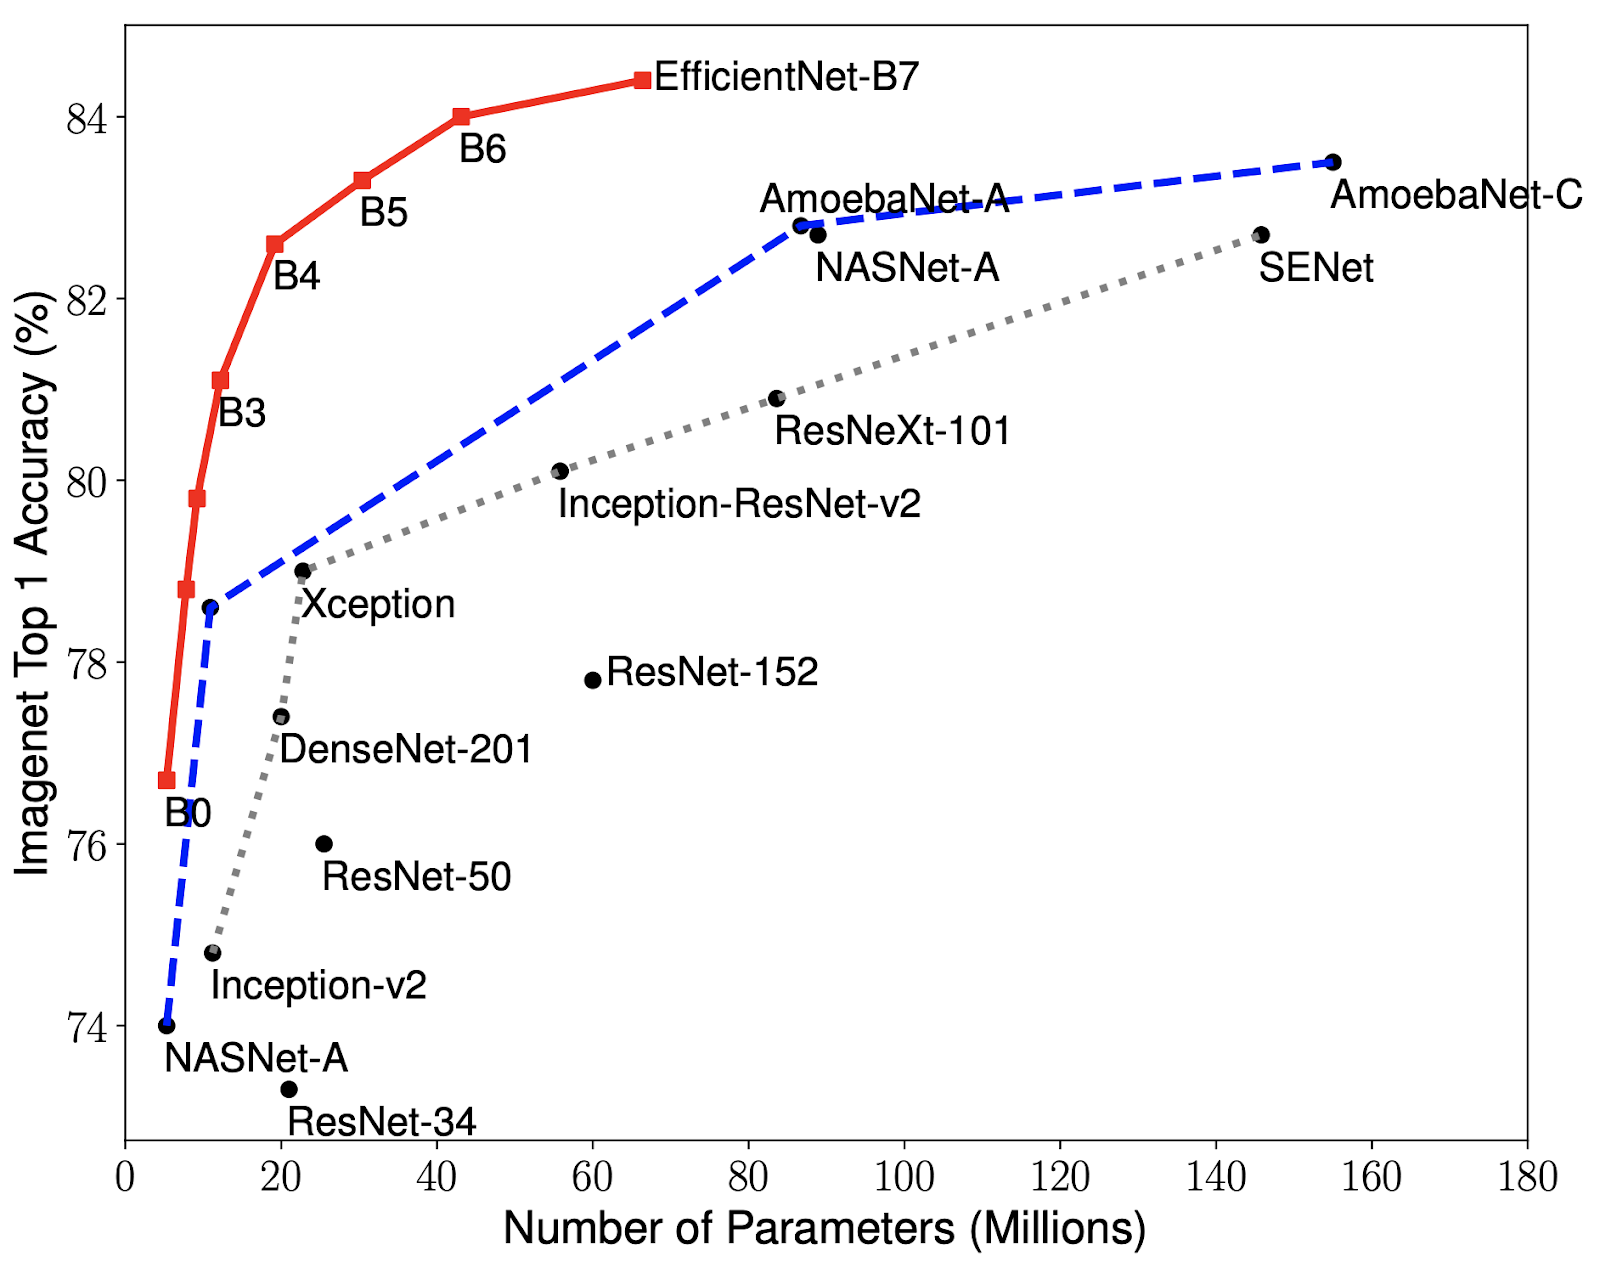
\includegraphics[scale=0.15]{Plot/efficientnet.png}
            \caption{Performance di EfficientNet rispetto ad altre reti.}
            \label{fig:efficientnet}
        \end{figure}
        
        Inoltre, i pesi importati, sono quelli ottenuti tramite la tecnica di training Noisy Student. Noisy Student è una metodo di apprendimento semi-supervisionato che si basa sull'allenare un modello (teacher) con immagini etichettate, utilizzarlo per etichettare nuove immagini e allenare un nuovo modello (student), della stessa grandezza o maggiore, con le immagini iniziali e quelle nuove ottenute dal primo modello aggiugendo del rumore. Questi passi vengono poi ripetuti più volte, invertendo teacher e student. Attraverso questa tecnica, utilizzando 300 milioni di immagini non etichettate, EfficientNet-B7 "Noisy Student" ha raggiunto una top-1 accuracy su ImageNet pari al 88.4\%. Questo approccio è stato scelto inoltre perché consente una generalizzazione migliore. \cite{xie2020selftraining}

        In coda alla rete pre-allenata importata, sono stati aggiunti dei layer fully-connected per adattare il modello al problema di regressione di PetFinder.my, mentre in testa alla rete è stato aggiunto un layer di preprocessing dei dati per rendere le immagini adatte ad essere trattate da EfficientNet. Di seguito
        è specificata l'architettura della sezione aggiunta:
        \begin{itemize}
            \item \textbf{Dense} - 1024 neuroni, ReLU
            \item \textbf{Dropout} - 50\% dei neuroni eliminati.
            \item \textbf{Dense} - 512 neuroni, ReLU
            \item \textbf{Dropout} - 30\% dei neuroni eliminati.
            \item \textbf{Dense} - 128 neuroni, ReLU
            \item \textbf{Dropout} - 10\% dei neuroni eliminati.
            \item \textbf{Dense} - 1 neurone, Linear
        \end{itemize}

        La funzione di loss scelta è stata la Mean Squared Error, mentre per monitorare le performance è stata utilizzata come metrica la Root Mean Squared Error. Come algoritmo di ottimizzazione è stato selezionato Adam.

    \subsection{Fully-connected neural network}
    \label{mlp}
    Per trattare i metadati riguardati le foto, si è deciso di utilizzare una rete neurale classica fully-connected. Di seguito viene 
    riportata l'architettura del modello:
    \begin{itemize}
        \item \textbf{Dense} - 32 neuroni, ReLU
        \item \textbf{Dropout} - 20\% dei neuroni eliminati.
        \item \textbf{Dense} - 8 neuroni, ReLU
        \item \textbf{Dropout} - 10\% dei neuroni eliminati.
        \item \textbf{Dense} - 1 neurone, Linear
    \end{itemize}

    Anche in questo caso, come per la rete convoluzionale, si sono utilizzate MSE come funzione di loss, RMSE come metrica delle performance del modello e Adam come algoritmo di ottimizzazione.

    \subsection{Hybrid DNN}
    \label{mulinput}
    L'ipotesi secondo cui predizioni più accurate si possono ottenere combinando le informazioni derivanti dalle foto degli animali e dai metadati ad esse allegati, ha portato alla
    costruzione di un terzo modello, combinazione dei due precedentemente descritti.

    Il modello in questione si presenta come una rete neurale ibrida \cite{yuan2020hybriddnns}, costituita dalla rete convoluzionale illustrata nel paragrafo \ref{cnn} e dalla rete fully-connected di cui si indicano le specifiche nel paragrafo \ref{mlp}, i quali output vengono concatenati e processati da due ulteriori layer.
    L'architettura proposta è mostrata in figura \ref{fig:model} nell'appendice A.


    \subsection{Addestramento}
    L'addestramento del modello finale descritto nel paragrafo \ref{mulinput}, è avvenuto allenando prima separatamente i due modelli di cui è composto. Entrambe le reti sono state allenate utilizzando una grandezza di batch di 32, per un massimo di 30 epoche, usando in entrambi i casi dei checkpoint basati sul valore minore di validation loss per evitare casi di overfitting. 

    I due modelli allenati sono stati successivamente uniti per andare a formare la rete ibrida e i loro pesi sono stati bloccati, così da poter effettuare il training 
    solo sulla sezione aggiunta in seguito alla concatenzaione dei risultati.
    Il modello ibrido è stato allenato con grandezza di batch pari a 32, per un massimo di 30 epoche, anche in questo caso utilizzando dei checkpoint.


\section{Risultati e Valutazione}

La metrica usata per la valutazione delle performance, essendo un task di regressione, è rappresentata dal calcolo del \textbf{RMSE (Root Mean Square Error)}:
\begin{equation}
    \textrm{RMSE} = \sqrt{\frac{1}{n} \sum_{i=1}^{n} (y_i - \hat{y}_i)^2} 
\end{equation}

con $\hat{y}_i$ il valore di popolarità predetto e $y_i$ il valore originale.


Le performance vengono valutate nelle varie epoche, sia sul training set che sul validation set. Tale valutazione viene effettuata prima sui singoli modelli e successivamente sul modello finale, ottenuto tramite la concatenazione dei primi due. E' possibile notare, in figura \ref{fig:rmse-all} come nella rete finale non ci sia traccia di overfitting, a differenza del modello ottenuto dalla rete convoluzionale in cui, sul train set, lo score continua a decrescere con un peggioramento sul validation set. 
Nella tabella \ref{table:rmse} vengono raffigurati i valori migliori ottenuti sul validation set per le varie architetture.

\begin{table}[H]
\caption{Confronto performance ottenute tra i diversi modelli sul validation set.}
  \vspace{3mm}
\centering
\begin{tabular}{|c|c|c|}
\hline
\textbf{Modello} & \textbf{RMSE Validation} & \textbf{MSE Loss} \\ \hline \hline
CNN     & 17.56           & 308.307  \\ \hline 
MLP     & 20.12           & 404.98   \\ \hline 
Hybrid  & 17.31           & 299.74   \\ \hline
\end{tabular}
\label{table:rmse}
\end{table}

\vspace{1cm}

\begin{figure}[h]
    \centering
    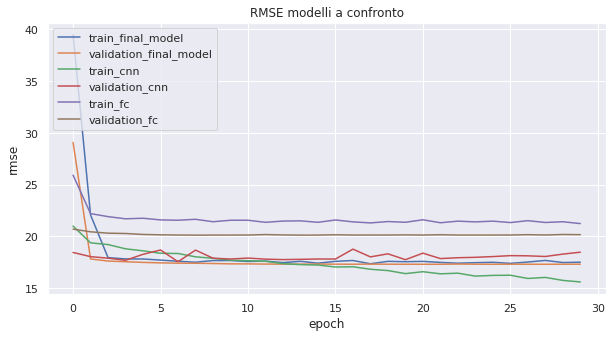
\includegraphics[width=13cm, height=6.5cm]{Plot/ALL_RMSE.png}
    \caption{RMSE modelli a confronto.}
    \label{fig:rmse-all}
\end{figure}


\subsection{Grad CAM}

Un problema noto del deep learning è rappresentato dal fatto che i modelli creati siano "black box", ovvero che sia difficilmente spiegabile come realmente le informazioni siano trattate all'interno dei vari layer. Per analizzare i risultati ottenuti è stato ritenuto opportuno effettuare un ulteriore studio su come la rete convoluzionale ragionasse sulle immagini per ottenere lo score di popolarità. Questo è possibile utilizzando lo strumento \textbf{Grad CAM}\cite{2019}. Tale metodo consente di produrre una spiegazione visiva di ciò che la rete osserva, determinando quali sono gli aspetti e le feature che più influenzano lo score finale. E' possibile notare nella figura \ref{fig:grad-cam} come la rete si vada a focalizzare maggiormente sull'animale nel caso in cui l'immagine risulti pulita da oggetti di disturbo; al contrario, se l'immagine presenta disturbi di vario genere, la rete andrà a dare maggior importanza all'ambiente circostante piuttosto che al solo animale.

\vspace{1cm}

\begin{figure}[h]
        \centering
        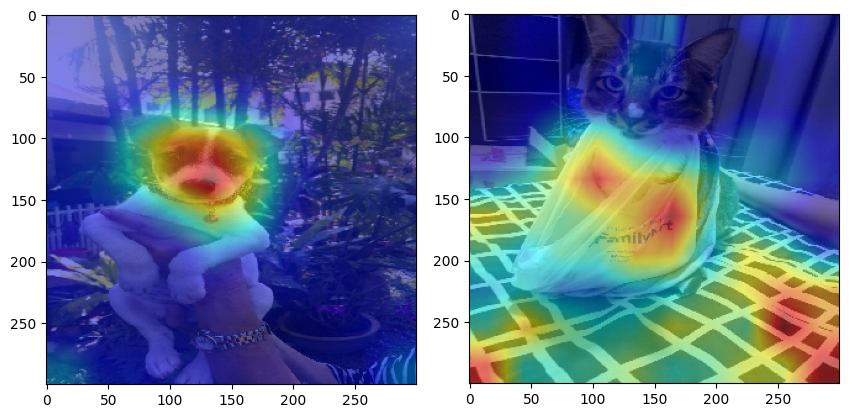
\includegraphics[scale=0.6]{Plot/GRAD-CAM.png}
        \caption{Confronto tra due Grad CAM ottenute da immagini con diversi score: quella di sinistra con popolarità più alta, mentre quella di destra più bassa.}
        \label{fig:grad-cam}
\end{figure}
    


\section{Considerazioni}

I risultati mostrano come le performance ottenute dal modello finale siano migliori di quelle ottenute tramite il solo fine-tuning sulla rete Efficient-Net B3 e nettamente migliori di quelli del Multilayer Perceptron sui meta-dati. Questo è probabilmente dovuto da un utilizzo combinato di tutte le informazioni disponibili: il layer fully-connected del modello finale riesce a dare i giusti pesi alle informazioni ottenute dalla rete convoluzionale, per le immagini, e da quella fully-connected, per i meta-dati, migliorando il risultato finale. Le performance ottenute risultano migliori di quelle raggiunte da altri team Kaggle che utilizzano reti convoluzionali allo stato dell'arte. I migliori risultati tuttavia vengono ottenuti da team che sfruttano un altro tipo di modello, ovvero i \textbf{transformer}, migliorando lo score finale di un punto di RMSE rispetto all'utilizzo di reti convoluzionali.


\section{Conclusioni e sviluppi futuri}
L'obiettivo di questo caso di studio è stato determinare se, l'uso congiunto di diversi modelli su tipologie di dati differenti, potesse effettivamente portare  a migliori risultati rispetto ai singoli.

L'ipotesi formulata, sebbene non supportata da una grande quantità di materiale presente in letteratura, è stata confermata empiricamente dai risultati ottenuti portando ad un miglioramento significativo delle performance. Tuttavia i risultati ottenuti non sono competitivi rispetto a quelli derivanti dall'utilizzo di nuove tecniche avanzate, quali transformer.

Un possibile sviluppo futuro, può essere la sostitusione della rete convoluzionale con un transformer e l'utilizzo di una risoluzione maggiore per le immagini, migliorie che devono essere necessariamente supportate da un hardware adeguato.

\bibliographystyle{IEEEtran}
\bibliography{references.bib}

\appendix
\section{Modello della rete}
\begin{figure}[H]
    \centering
    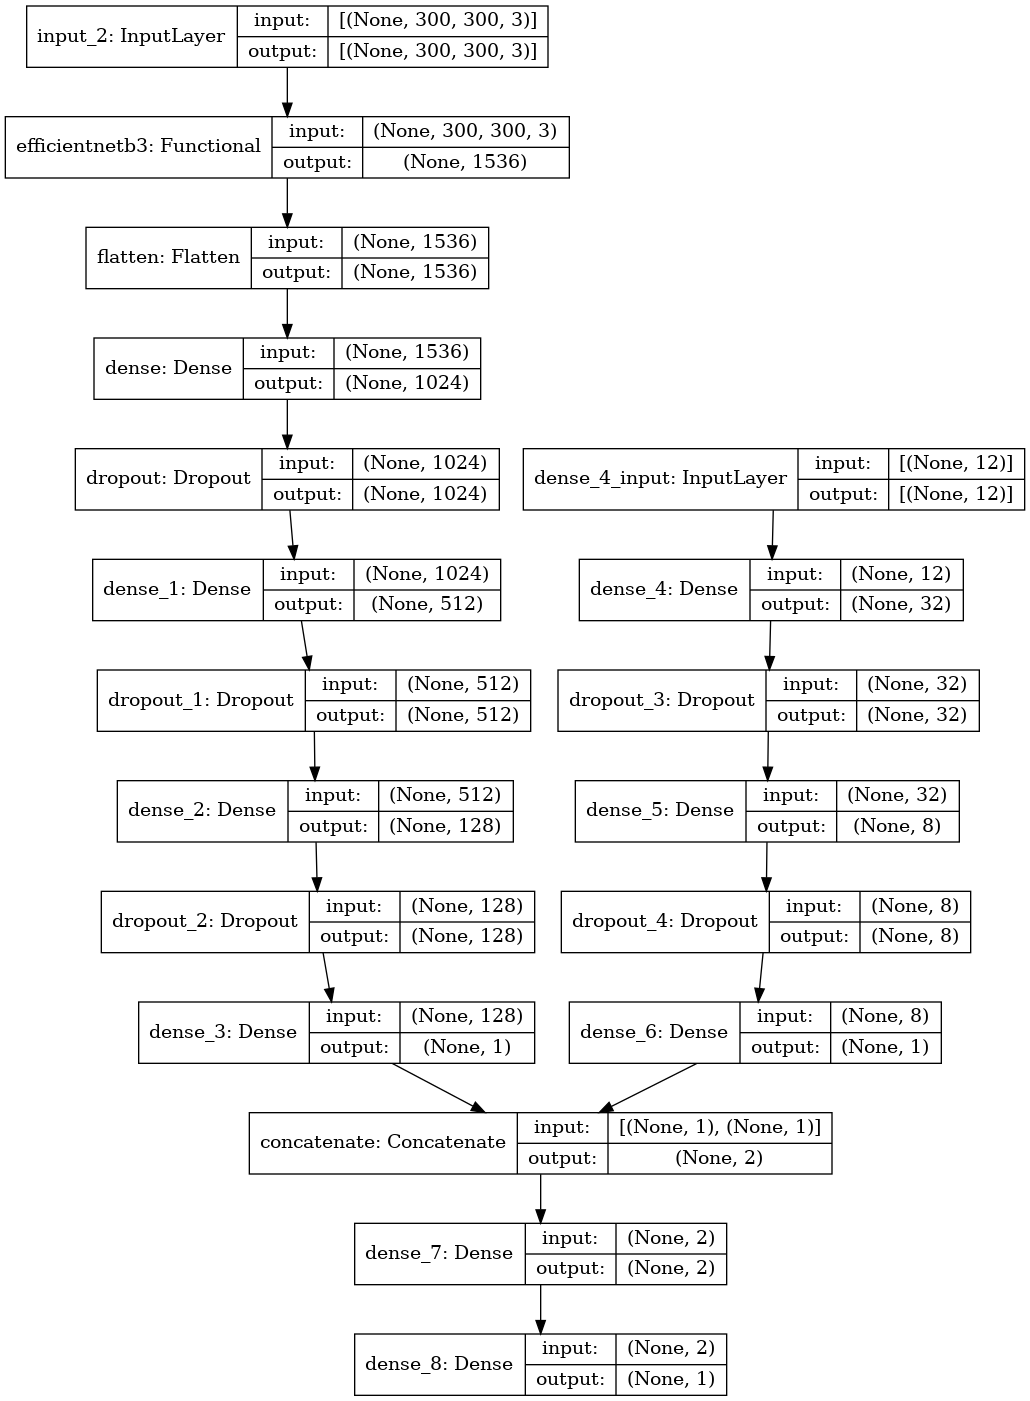
\includegraphics[scale=0.33]{Plot/Model-Plot.png}
    \caption{Architettura Hybrid DNN}
    \label{fig:model}
\end{figure}

\end{document}